\documentclass[UTF8]{ctexart}
\usepackage{geometry}
\usepackage{indentfirst}
\usepackage{hyperref}
\usepackage{harpoon}
\usepackage{amsmath}
\usepackage{graphicx}
\usepackage{float}
\usepackage{subfigure}
\usepackage{multirow}
\usepackage{array}
\usepackage{tikz}
\usetikzlibrary{arrows, shapes, positioning, calc}
\geometry{a4paper, left=1cm, right=1cm, top=2cm, bottom=2cm}
\setlength{\parindent}{1cm}
\renewcommand\contentsname{Content}
\CTEXoptions[today=old]
\title{Report 1: Pseudopotential}
\author{Yuanxing Duan 段元兴}
\date{\today}
\begin{document}
\maketitle
\thispagestyle{empty}
\setcounter{page}{1}
\newpage
\tableofcontents
\newpage
    \section{Introduction to pseudopotential}
        \indent A pseudopotential (effective potential) is used as an approximation for the simplified description
        of complex systems. For example, replacing the complex core elections and nucleus inside an atomic with a
        simplified potential $V_{pseudo}$ so that Schrödinger equation contains a modified effective potential term
        instead of the Coulombic potential term for core electrons normally found in the Schrödinger equation. In
        this way the core states are eliminated and the valence elections are described by pseudo-wavefunctions $\psi_{pseudo}$
        with significantly fewer nodes. And because the core electrons are usually more local, so require more
        higher energy plane waves in the basis set, which means higher cutoff energy $E_{cut}=\dfrac{\hbar^2G_{cut}^2}{2m}$.
        With pseudopotential we can ignore these so valence elections + pseudopotential are much more efficient than
        considering all electrions.\\
        First-principles pseudopotentials are derived from an atomic reference state, requiring that the pseudo and all
        electron valence eigenstates have the same energies and amplitude (and thus density) outside a chosen core cut-off
        radius $r_c$. And thus there are two approximation:\\
        \indent 1. It's a picture of one election.\\
        \indent 2. The small-core approximation assumes that there is no significant overlap between core and valence wavefunction.\\
    \section{Useful pseudopotentials}
        \indent Norm-conserving and ultrasoft are the two most common forms of pseudopotential used in modern plane-wave electronic
        structure codes. They allow a basis-set with a significantly lower cut-off (the frequency of the highest Fourier mode) to be
        used to describe the electron wavefunctions and so allow proper numerical convergence with reasonable computing resources.
        \subsection{Norm-conserving pseudopotential}
            \indent Norm-conserving pseudopotential was first proposed by Hamann, Schlüter, and Chiang (HSC) in 1979. The original HSC
            norm-conserving pseudopotential takes the following form:
            \begin{equation}
                \hat{V}_{ps}(r)=\sum_l\sum_m|Y_{lm}\rangle V_{lm}(r)\langle Y_{lm}|
            \end{equation}
            where $|Y_{lm}\rangle$ projects a one-particle wavefunction, such as one Kohn-Sham orbital, to the angular momentum labeled by
            $\{l,m\}$. $V_{lm}(r)$ is the pseudopotential that acts on the projected component. Different angular momentum states then feel
            different potentials, thus the HSC norm-conserving pseudopotential is non-local, in contrast to local pseudopotential which acts
            on all one-particle wavefunctions in the same way. Norm-conserving pseudopotentials are constructed to enforce three conditions:\\
            \indent 1. Inside the cut-off radius $r_c$, the norm of each pseudo-wavefunction be identical to its corresponding all-electron wavefunction:
            \begin{equation}
                \int_0^{r_c}dr^3\phi_{\mathbf{R},i}({\vec{r}})\phi_{\mathbf{R},j}({\vec{r}})=
                \int_0^{r_c}dr^{3}{\tilde{\phi}}_{\mathbf{R},i}({\vec{r}}){\tilde{\phi}}_{\mathbf{R},j}({\vec{r}})
            \end{equation}
            where $\phi_{\mathbf{R},i}$ and $\tilde{\phi}_{\mathbf{R},i}$ are the all-electron and pseudo reference states for the pseudopotential
            on atom $\mathbf{R}$. This is because the total charge in the core region should be the same as the real situation.\\
            \indent 2. All-election and pseudo wavefunctions are identical outside cutoff radius $r_c$.\\
            \indent 3. Pseudo wavefunctions $\phi_{\mathbf{R},i}$ should be nodeless.\\
            \indent In this way the pseudopotential inside $r_c$ correctly mimics the scattering property of the full potential at the eigenvalue energy.
        \subsection{Ultrasoft pseudopotential}
            \indent The development of first-principles norm-conserving pseudopotentials has paved the way to accurate calculations of solid-state
            properties within the local-density approximation using plane-wave basis functions. However, the utility of this approach to systems containing
            highly localized valence orbitals has been limited, because of the difficulty of representing the pseudo wavefunctions in a plane-wave basis.\\
            The basis set size can be reduced to some extent by constructions which insure optimal smoothness of the potential or wave function and by
            moving the cutoff radius outward. However, the normconserving condition requires that the total pseudocharge inside the core match that of the
            all-electron (AE) wave function. Thus for many important cases it has proven impossible to construct a pseudo wavefunction which is much smoother than the AE one.\\
            The construction of ultrasoft pseudopotential is:\\
            \indent 1. Generate a smooth local potential $V_{loc}(r)$ which approaches $V_{AE}(r)$ beyond $r_c^{loc}$.\\
            \indent 2. Like norm-conserving pseudoptentials, construct pseudo wavefunctions subject to the constraints that it join smoothly to $\psi_i$ (All-election wavefunction)
            at $r_c$ and satisfy the norm-conserving property $\langle\phi_i|\phi_i\rangle_R=\langle\psi_i|\psi_i\rangle_R$. Now the wavefunction
            \begin{equation}
                |\chi_i\rangle=(\varepsilon_i-T-V_{loc})|\phi_i\rangle
            \end{equation}
            is local since it vanishes at and beyond $R$ where $V_{AE}=V_{loc}$ and $\phi_i=\psi_i$. and the nonlocal pseudopotential operator
            \begin{equation}
                V_{NL}=\dfrac{|\chi_i\rangle\langle\chi_i|}{\langle\chi_i|\phi_i\rangle}
            \end{equation}
            is well defined. It is straightforward to verify that $|\phi_i\rangle$ is an eignevector of $T+V_{loc}+V_{NL}$
            \begin{equation}
                (T+V_{loc}+V_{NL})|\phi_i\rangle=(\varepsilon_i+V_{NL})|\phi_i\rangle-|\chi_i\rangle=\varepsilon_i|\phi_i\rangle
            \end{equation}
            and the scattering properties and their energy derivatives are correct at $\varepsilon_i$ in the usual way.\\
            \indent 3. Generalizing the previous construction to the case of two or more energies $\varepsilon_i$at which scatting properties will be correct. For a given
            angular momentum $l$, some number (usually 1, 2 or 3) of energies which span the energy of occupied states of a target calculation are chosen. Now we expect that
            the set of pseudo wavefunctions $|\phi_i\rangle$, which were constructed from $|\psi_i\rangle$ but may not satisfy the generalized nrom-conserving condition ($Q_{ij}=0$):
            \begin{equation}
                Q_{ij}=\langle\psi_i|\psi_j\rangle_R-\langle\phi_i|\phi_j\rangle_R.
            \end{equation}
            Forming the matrix $B_{ij}=\langle\phi_i|\chi_j\rangle$ and defining a set of local wavefunctions
            \begin{equation}
                |\beta_i\rangle=\sum_j(B^{-1})_{ji}|\chi_j\rangle.
            \end{equation}
            which are dual to the $|\phi_i\rangle$. The nonlocal pseudopotential operator can be chosen as
            \begin{equation}
                V_{NL}=\sum_{i,j}B_{ij}|\beta_i\rangle\langle\beta_j|.
            \end{equation}
            Then we can show that
            \begin{equation}
                \begin{array}[h]{ll}
                    (H-\varepsilon_i)|\phi_i\rangle&=(T+V_{loc}+V_{NL}-\varepsilon_i)|\phi_i\rangle\\
                    &=V_{NL}|\phi_i\rangle-|\chi_i\rangle\\
                    &=\sum_{j,k}B_{jk}\langle\beta_k|\phi_i\rangle|\beta_j\rangle-|\chi_i\rangle\\
                    &=\sum_{j,k}B_{jk}\sum_l(B^{-1})^*_{lk}\langle\chi_l|\phi_i\rangle|\beta_j\rangle-|\chi_i\rangle\\
                    &=\sum_{j,k}B_{jk}\sum_l(B^{-1})^*_{lk}B_{il}^*|\beta_j\rangle-|\chi_i\rangle\\
                    &=\sum_{j,k}B_{jk}\delta_{ik}|\beta_j\rangle-|\chi_i\rangle\\
                    &=\sum_{j}B_{ji}|\beta_j\rangle-|\chi_i\rangle\\
                    &=\sum_{j}B_{ji}\sum_k(B^{-1})_{kj}|\chi_k\rangle-|\chi_i\rangle\\
                    &=\sum_{k}\sum_j(B^{-1})_{kj}B_{ji}|\chi_k\rangle-|\chi_i\rangle\\
                    &=\sum_{k}\delta_{ki}|\chi_k\rangle-|\chi_i\rangle\\
                    &=0
                \end{array}
            \end{equation}
            \indent 4. Define a nonlocal overlap operator
            \begin{equation}
                S=1+\sum_{i,j}Q_{ij}|\beta_i\rangle\langle\beta_j|
            \end{equation}
            and redefine the nonlocal potential operator to be
            \begin{equation}
                V_{NL}=\sum_{i,j}D_{ij}|\beta_i\rangle\langle\beta_j|=\sum_{i,j}(B_{ij}+\varepsilon_jQ_{ij})|\beta_i\rangle\langle\beta_j|.
            \end{equation}
            Notice that
            \begin{equation}
                \langle\phi_i|S|\phi_j\rangle_R=\langle\phi_i|\phi_j\rangle_R+\sum_{i,j}Q_{ij}\langle\phi_i|\beta_i\rangle_R\langle\beta_j|\phi_j\rangle_R
                =\langle\psi_i|\psi_j\rangle_R
            \end{equation}
            Then $|\phi_i\rangle$ is easily shown to be a solution of the generalized eigenvalue problem $(H-\varepsilon_iS)|\phi_i\rangle=0$.\\
            \indent The relaxation of the constraint $Q_{ij}=0$ means that each $\psi_i$ can be made into a pseudo wavefunction $\phi_i$ independently with the only
            constraint which is matching $\phi(r)$ to $\psi(r)$ at the cutoff radius. Thus it becomes possible to choose the cutoff radius to be well beyond
            the radial wavefunction maximum.
            \begin{center}
                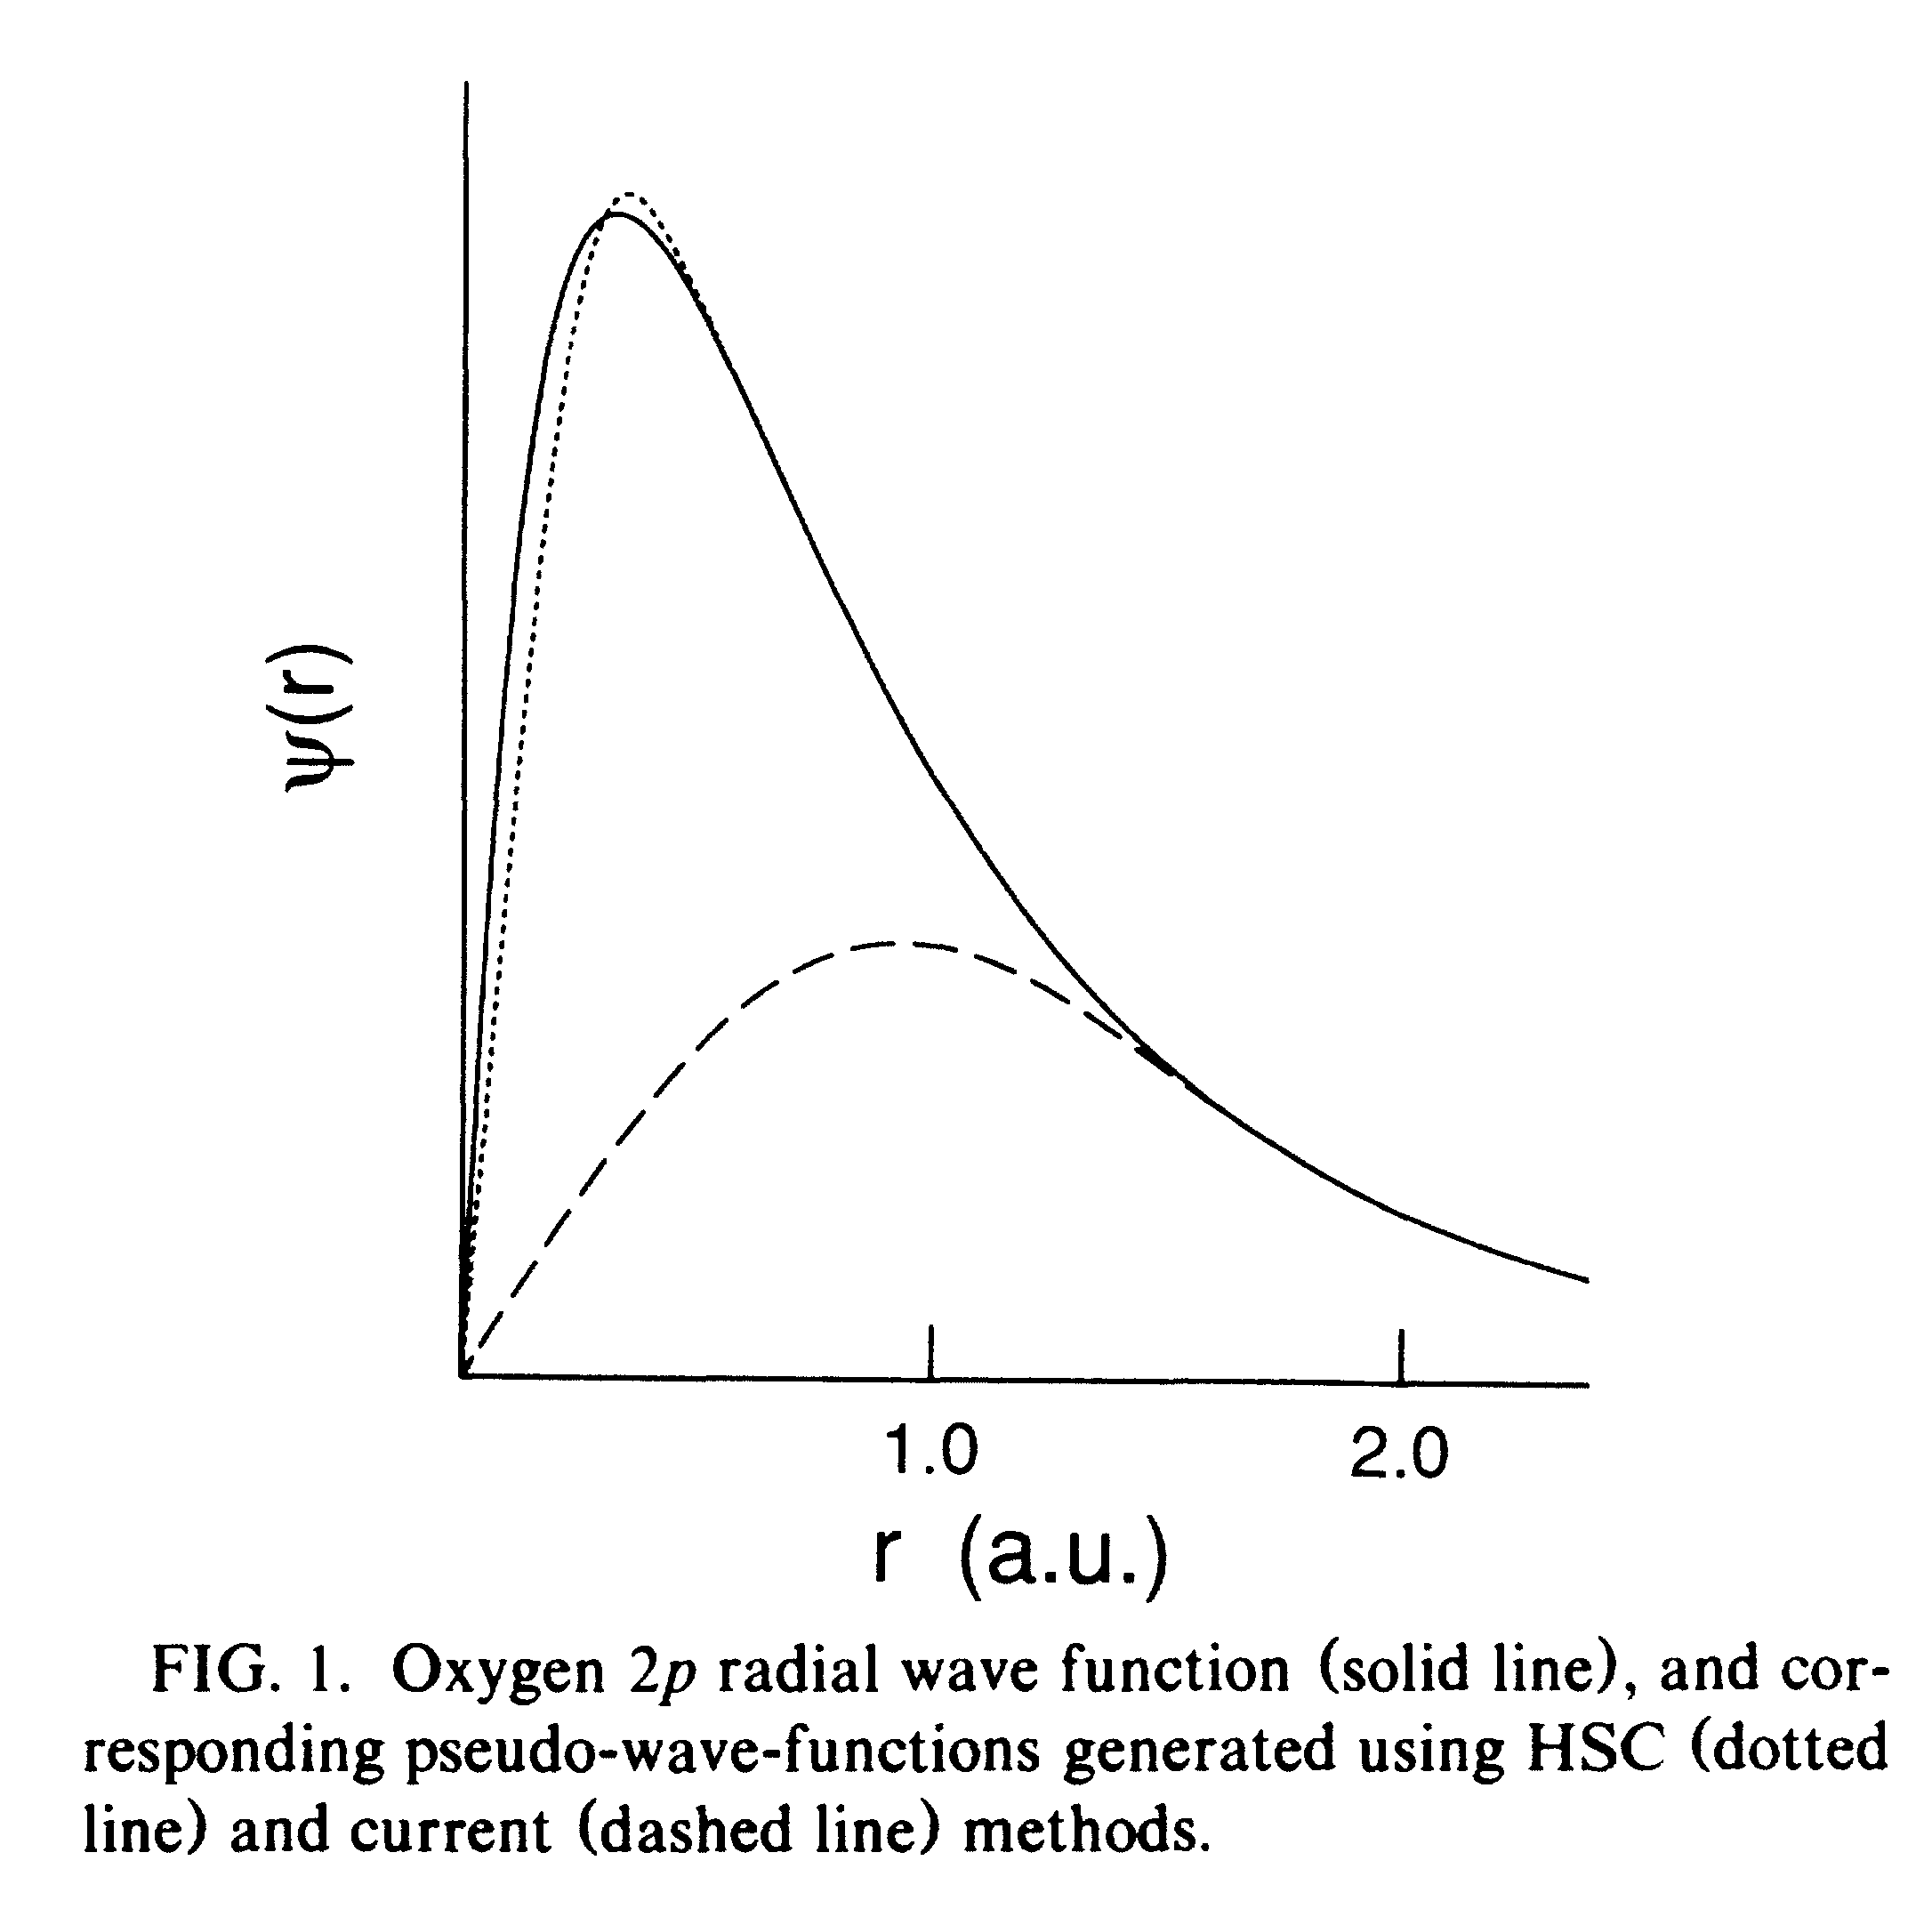
\includegraphics[width = 8cm]{1.png}
            \end{center}
\end{document}